\documentclass{report}

\usepackage[warn]{mathtext}
\usepackage[T2A]{fontenc}
\usepackage[utf8]{luainputenc}
\usepackage[english, russian]{babel}
\usepackage[pdfpagemode=UseNone,colorlinks,allcolors=black]{hyperref}
\usepackage{tempora}
\usepackage[12pt]{extsizes}
\usepackage{listings}
\usepackage{color}
\usepackage{geometry}
\usepackage{enumitem}
\usepackage{multirow}
\usepackage{graphicx}
\usepackage{indentfirst}
\usepackage{amsmath}
\usepackage{soul}

\sethlcolor{gray}

\geometry{a4paper,top=2cm,bottom=2cm,left=2.5cm,right=1.5cm}
\setlength{\parskip}{0.5cm}
\setlist{nolistsep, itemsep=0.3cm,parsep=0pt}

\usepackage{listings}
\lstset{language=C++,
        basicstyle=\footnotesize,
		keywordstyle=\color{blue}\ttfamily,
		stringstyle=\color{red}\ttfamily,
		commentstyle=\color{green}\ttfamily,
		morecomment=[l][\color{red}]{\#}, 
		tabsize=4,
		breaklines=true,
  		breakatwhitespace=true,
  		title=\lstname,       
}

\makeatletter
\renewcommand\@biblabel[1]{#1.\hfil}
\makeatother

\begin{document}

\begin{titlepage}

\begin{center}
Министерство науки и высшего образования Российской Федерации
\end{center}

\begin{center}
Федеральное государственное автономное образовательное учреждение высшего образования \\
Национальный исследовательский Нижегородский государственный университет им. Н.И. Лобачевского
\end{center}

\begin{center}
Институт информационных технологий, математики и механики
\end{center}

\vspace{4em}

\begin{center}
\textbf{\LargeОтчет по лабораторной работе} \\
\end{center}
\begin{center}
\textbf{\Large<<Сортировка Шелла с простым слиянием>>} \\
\end{center}

\vspace{4em}

\newbox{\lbox}
\savebox{\lbox}{\hbox{text}}
\newlength{\maxl}
\setlength{\maxl}{\wd\lbox}
\hfill\parbox{7cm}{
\hspace*{5cm}\hspace*{-5cm}\textbf{Выполнил:} \\ студент группы 3821Б1ПР1\\Юрин А. Ю.\\
\\
\hspace*{5cm}\hspace*{-5cm}\textbf{Преподаватель:}\\ кандидат технических наук\\Сысоев А. В.\\
}
\vspace{\fill}

\begin{center} Нижний Новгород \\ 2023 \end{center}

\end{titlepage}

\setcounter{page}{2}

% Содержание
\tableofcontents
\newpage

% Введение
\section*{Введение}
\addcontentsline{toc}{section}{Введение}
\par Сортировка является одной из типовых проблем обработки данных и обычно понимается как задача размещения элементов неупорядоченного набора значений. Существует множество алгоритмов сортировок с различной алгоритмической сложностью и с различным объёмом используемой дополнительной памяти.

\par Целью данной лабораторной работы является реализация сортировки Шелла с простым слиянием с использованием MPI.

\newpage

% Постановка задачи
\section*{Постановка задачи}
\addcontentsline{toc}{section}{Постановка задачи}
\par \textbf{В рамках данного задания нужно выполнить следующие задачи:}
\begin{enumerate}
    \item Реализовать две версии алгоритма сортировки Шелла:
    \begin{itemize}
    \item Последовательная реализация - алгоритм выполняется в одном процессе.
    \item Параллельная реализация - алгоритм выполняется в нескольких процессах. 
    \end{itemize}
    \item Сравнить производительность последовательной и параллельной версий.
    \item Провести анализ полученных данных.
\end{enumerate}
\newpage

% Описание алгоритма
\section*{Описание алгоритма}
\addcontentsline{toc}{section}{Описание алгоритма}
\par Сортировка Шелла (англ. Shell sort) — алгоритм сортировки, являющийся усовершенствованным вариантом сортировки вставками. Идея метода Шелла состоит в сравнении элементов, стоящих не только рядом, но и на определённом расстоянии друг от друга. Иными словами — это сортировка вставками с предварительными «грубыми» проходами.

\par \textbf{Алгоритм:}

\begin{enumerate}
    \item Cравниваем и сортируем между собой значения, стоящие один от другого на некотором расстоянии ${d}$.
    \item Повторяем для некоторых меньших значений ${d}$.
    \item Завершаем сортировку Шелла упорядочиванием элементов при ${d = 1}$.
\end{enumerate}

\par \textbf{Выбор длины промежутков:}
\par Среднее время работы алгоритма зависит от длин промежутков — ${d}$, на которых будут находиться сортируемые элементы исходного массива ёмкостью ${N}$ на каждом шаге алгоритма.

\newpage

% Описание схемы распараллеливания
\section* {Описание схемы распараллеливания}
\addcontentsline{toc}{section}{Описание схемы распараллеливания}
\par \textbf{Шаги:} 
\begin{enumerate}
    \item Разделяем массив на ${N}$ приблизительно равных частей и рассылаем каждому процессу по части,  используя boost::mpi::scatterv
    \item Каждый процесс сортирует свою часть массива сортировкой Шелла.
    \item Собираем отсортированные части массива в один массив:
    \begin{itemize}
        \item Части массива собираются в 0-м процессе при помощи boost::mpi::gatherv. 0-ой процесс сортирует собранный массив сортировкой слияния.
        \item Части массива собираются в виде дерева при помощи  boost::mpi::send и  boost::mpi::recv, т.е. процесс с нечётным номером (номер - это порядковое число среди процессов, содержащих отсортированную часть, не ранг процесса) отправляет массив следующему по номеру процессу, если такой существует. Таким образом, части массива сортируются парами сортировкой слияния. И в итоге отсортированный массив получается в (${N-1}$) процессе и отправляется в 0-ой процесс.
        
%    \begin{figure}[h]
%            \centering
%           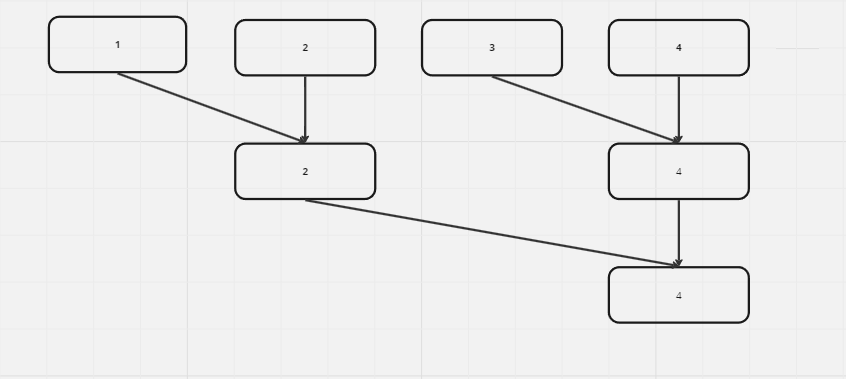
\includegraphics[width=1\textwidth]{tree.png}
%           \caption{Схема сбора отсортированных частей массива на примере 4-х процессов}
%            \label{fig:моя_картинка}
%       \end{figure}
    \end{itemize}
\end{enumerate}

\newpage

% Результаты экспериментов
\section*{Результаты экспериментов}
\addcontentsline{toc}{section}{Результаты экспериментов}
Для проведения экспериментов по вычислению эффективности работы алгоритмов использовалась система со следующей конфигурацией:
\begin{itemize}
\item Процессор: m2 pro 10 ядер CPU, 16 ядер GPU;
\item Оперативная память: 16гб;
\item Операционная система: macOS Sonoma.
\end{itemize}

\par \textbf{Входные данные:} \url{https://disk.yandex.ru/d/cqeFGT4iy_L9Zg}
\par \textbf{Результаты экспериментов:}
\begin{center}
\begin{tabular}{ ||c | c | c ||  }
    \hline
    \multicolumn{3}{| c |}{Запуск алгоритма на 1-м процессе}\\
    \hline Последовательный (сек) & Параллельный 1 (сек) & Параллельный 2 (сек)\\ \hline
    5.92553 & 6.16595 & 6.13308 \\ \hline
\end{tabular}\\[5mm]

\begin{tabular}{ ||c | c | c ||  }
    \hline
    \multicolumn{3}{| c |}{Запуск алгоритма на 2-х процессах}\\
    \hline Последовательный (сек) & Параллельный 1 (сек) & Параллельный 2 (сек)\\ \hline
    6.2653 & 3.43618 & 3.29032 \\ \hline
\end{tabular}\\[5mm]

\begin{tabular}{ ||c | c | c ||  }
    \hline
    \multicolumn{3}{| c |}{Запуск алгоритма на 3-х процессах}\\
    \hline Последовательный (сек) & Параллельный 1 (сек) & Параллельный 2 (сек)\\ \hline
    6.57329 & 2.64138 & 2.39503 \\ \hline
\end{tabular}\\[5mm]

\begin{tabular}{ ||c | c | c ||  }
    \hline
    \multicolumn{3}{| c |}{Запуск алгоритма на 4-х процессах}\\
    \hline Последовательный (сек) & Параллельный 1 (сек) & Параллельный 2 (сек)\\ \hline
    6.4043 & 2.40572 & 1.83424 \\ \hline
\end{tabular}\\[5mm]

\begin{tabular}{ ||c | c | c ||  }
    \hline
    \multicolumn{3}{| c |}{Запуск алгоритма на 5-и процессах}\\
    \hline Последовательный (сек) & Параллельный 1 (сек) & Параллельный 2 (сек)\\ \hline
    6.42166 & 2.41869 & 1.82969 \\ \hline
\end{tabular}\\[5mm]

\begin{tabular}{ ||c | c | c ||  }
    \hline
    \multicolumn{3}{| c |}{Запуск алгоритма на 6-и процессах}\\
    \hline Последовательный (сек) & Параллельный 1 (сек) & Параллельный 2 (сек)\\ \hline
    6.45266 & 2.4226 & 1.52497 \\ \hline
\end{tabular}\\[5mm]

\begin{tabular}{ ||c | c | c ||  }
    \hline
    \multicolumn{3}{| c |}{Запуск алгоритма на 7-и процессах}\\
    \hline Последовательный (сек) & Параллельный 1 (сек) & Параллельный 2 (сек)\\ \hline
    6.5211 & 2.62462 & 1.48207 \\ \hline
\end{tabular}\\[5mm]

\begin{tabular}{ ||c | c | c ||  }
    \hline
    \multicolumn{3}{| c |}{Запуск алгоритма на 8-и процессах}\\
    \hline Последовательный (сек) & Параллельный 1 (сек) & Параллельный 2 (сек)\\ \hline
    6.52086 & 2.86034 & 1.44206 \\ \hline
\end{tabular}\\[5mm]

\end{center}

\newpage

% Анализ результатов
\section*{Анализ результатов}
\addcontentsline{toc}{section}{Анализ результатов}
Посчитаем средние коэффициенты ускорения по формуле $ p_i = \frac{T_{si}}{T_{pi}} $, где $T_{si}$ - время последовательного алгоритма, а $T_{pi}$ время параллельного алгоритма для {i} задачи, где $i = {2, ..., 8}$. \\

Получаем следующие результаты:\\[2mm]

\begin{center}
\begin{tabular}{ ||c | c | c ||}
 \hline
 \multicolumn{3}{| c |}{Коэффициент ускорения}\\
 \hline
 Количество процессов & Ускорение 1 & Ускорение 2\\
 \hline
2 & 1.8 & 1.9 \\
3 & 2.49 & 2.7 \\
4 & 2.66 & 3.49 \\
5 & 2.66 & 3.51 \\
6 & 2.66 & 4.23 \\
7 & 2.48 & 4.4 \\
8 & 2.28 & 4.52 \\
 \hline
\end{tabular}
\end{center}

\textbf{Вывод}: 
    \begin{itemize}
        \item Части массива собираются в 0-м процессе: 
        \par После 4-х процессов с увеличением кол-ва процессов ускорение перестаёт расти, а после 7-ми - начинает уменьшаться.
        \item Части массива собираются в виде дерева:
        \par После 6-ти процессов с увеличением кол-ва процессов рост ускорения замедляется.
        \item Значения ускорения в каждом эксперименте находятся в корректном диапазоне.
        \item Параллельная версия значительно ускоряет работу алгоритма.
    \end{itemize}

\newpage

% Заключение
\section*{Заключение}
\addcontentsline{toc}{section}{Заключение}
Таким образом, в рамках данной лабораторной работы были реализованы последовательный и параллельный алгоритмы сортировки Шелла с простым слиянием. Проведенные замеры производительности доказали эффективность распараллеливания данного алгоритма.
\newpage

% Литература
\section*{Литература}
\addcontentsline{toc}{section}{Литература}
\begin{enumerate}
\item Wikipedia. URL: \newline \url{https://ru.wikipedia.org/wiki/%D0%A1%D0%BE%D1%80%D1%82%D0%B8%D1%80%D0%BE%D0%B2%D0%BA%D0%B0_%D0%A8%D0%B5%D0%BB%D0%BB%D0%B0}
\item Boost MPI. URL: \newline \url{https://www.boost.org/doc/libs/1_80_0/doc/html/mpi.html}
\end{enumerate}


\newpage

\section*{Приложение}
\addcontentsline{toc}{section}{Приложение}

\begin{lstlisting}[language=C++,caption=h файл]
// Copyright 2023 Yurin Andrey
#ifndef TASKS_TASK_3_YURIN_A_SHELL_SORT_SIMPLE_MERGE_SHELL_SORT_SIMPLE_MERGE_H_
#define TASKS_TASK_3_YURIN_A_SHELL_SORT_SIMPLE_MERGE_SHELL_SORT_SIMPLE_MERGE_H_

#include "vector"

bool IsSorted(std::vector<int> array);
std::vector<int> GetRandomVector(int  size, int minValue, int maxValue);
std::vector<int> MergeTwoSortedArrays(std::vector<int> firstArray, std::vector<int> secondArray);
void MergeTwoSortedArrays(std::vector<int>* array, int leftIndex, int midIndex, int rightIndex);
std::vector<int> ShellSortSequential(std::vector<int> array);
std::vector<int> ShellSortParallel(std::vector<int> array, bool combineInOneProcess = false);

#endif  // TASKS_TASK_3_YURIN_A_SHELL_SORT_SIMPLE_MERGE_SHELL_SORT_SIMPLE_MERGE_H_

\end{lstlisting}
\newpage
\begin{lstlisting}[language=C++,caption=cpp файл]

#include <random>
#include <algorithm>
#include <iterator>
#include <utility>
#include <boost/mpi/communicator.hpp>
#include <boost/mpi/collectives.hpp>
#include "task_3/yurin_a_shell_sort_simple_merge/shell_sort_simple_merge.h"

#define MAIN_PROCESS 0
#define DEFAULT_TAG 0

void CombineInOneProcess(
        const boost::mpi::communicator& world,
        std::vector<int>* array,
        const std::vector<int>& localArray,
        const std::vector<int>& sizes
) {
    boost::mpi::gatherv(world, localArray.data(), localArray.size(), array->data(), sizes, 0);

    if (world.rank() == 0) {
        int rightIndex = sizes[0] -1;
        for (int i = 1; i < sizes.size(); ++i) {
            int midIndex = rightIndex + 1;
            rightIndex += sizes[i];
            MergeTwoSortedArrays(array, 0, midIndex, rightIndex);
        }
    }
}

std::vector<int> RecalculateProcessesInvolved(std::vector<int> processesInvolved) {
    std::vector<int> newProcessesInvolved;

    for (auto iter = processesInvolved.begin(); iter != processesInvolved.end(); iter++) {
        if (std::distance(processesInvolved.begin(), iter) % 2 == 0) {
            if ((iter + 1) == processesInvolved.end()) {
                newProcessesInvolved.push_back(*(iter));
            }
        } else {
            newProcessesInvolved.push_back(*iter);
        }
    }
    return newProcessesInvolved;
}

void GetSortedArrayInNullProcess(
        const boost::mpi::communicator& world,
        std::vector<int>* array,
        const std::vector<int>& localArray
        ) {
    if (world.size() - 1 == 0)
        return;

    if (world.rank() == world.size() - 1) {
        world.send(MAIN_PROCESS, DEFAULT_TAG, localArray.data(), localArray.size());
    } else if (world.rank() == 0) {
        world.recv(world.size() - 1, DEFAULT_TAG, array->data(), array->size());
    }
    world.barrier();
}

void SendLocalArray(
        const boost::mpi::communicator& world,
        const std::vector<int>& localArray,
        const int& dest
        ) {
    world.send(dest, DEFAULT_TAG, localArray.size());
    world.send(dest, DEFAULT_TAG, localArray.data(), localArray.size());
}

void RecvLocalArrayAndSort(
        const boost::mpi::communicator& world,
        std::vector<int>* localArray,
        const int& dest
        ) {
    size_t sizeOfTempArray = 0;
    world.recv(dest, DEFAULT_TAG, sizeOfTempArray);
    std::vector<int> tempLocalArray(sizeOfTempArray);
    world.recv(dest, DEFAULT_TAG, tempLocalArray.data(), sizeOfTempArray);
    *localArray = MergeTwoSortedArrays(*localArray, tempLocalArray);
}

void OneStepForCombineByPair(
        const boost::mpi::communicator& world,
        std::vector<int>* localArray,
        const std::vector<int>& processesInvolved
        ) {
    auto iter = std::find(processesInvolved.begin(), processesInvolved.end(), world.rank());
    if (iter != processesInvolved.end()) {
        if (std::distance(processesInvolved.begin(), iter) % 2 == 0) {
            if ((iter + 1) != processesInvolved.end()) {
                SendLocalArray(world, *localArray, *(iter + 1));
            }
        } else {
            RecvLocalArrayAndSort(world, localArray, *(iter - 1));
        }
    }
}

void CombineByPair(
        const boost::mpi::communicator& world,
        std::vector<int>* array,
        std::vector<int> localArray
        ) {
    std::vector<int> processesInvolved;
    for (int i = 0; i < world.size(); ++i) {
        processesInvolved.push_back(i);
    }

    while (processesInvolved.size() > 1) {
        OneStepForCombineByPair(world, &localArray, processesInvolved);
        processesInvolved = RecalculateProcessesInvolved(processesInvolved);
        world.barrier();
    }

    GetSortedArrayInNullProcess(world, array, localArray);
}

bool IsSorted(std::vector<int> array) {
    for (int i = 0; i < array.size() - 1; ++i) {
        if (array[i] > array[i + 1]) {
            return false;
        }
    }
    return true;
}

std::vector<int> GetRandomVector(int size, int minValue, int maxValue) {
    std::random_device dev;
    std::mt19937 gen(dev());
    std::uniform_int_distribution<> distribution(minValue, maxValue);

    std::vector<int> vec(size);
    for (int  i = 0; i < size; i++) {
        vec[i] = distribution(gen);
    }
    return vec;
}

std::vector<int> MergeTwoSortedArrays(std::vector<int> firstArray, std::vector<int> secondArray) {
    std::vector<int> result(firstArray.size() + secondArray.size());

    for (int i = 0, j = 0; i + j < firstArray.size() + secondArray.size(); ) {
        if (i < firstArray.size() && j < secondArray.size()) {
            result[i + j - 1] = firstArray[i] < secondArray[j] ? firstArray[i++]: secondArray[j++];
        } else if (i < firstArray.size()) {
            result[i + j - 1] = firstArray[i++];
        } else {
            result[i + j - 1] = secondArray[j++];
        }
    }

    return result;
}

void MergeTwoSortedArrays(std::vector<int>* array, int leftIndex, int midIndex, int rightIndex) {
    std::vector<int> firstArray((*array).begin() + leftIndex, (*array).begin() + midIndex);
    std::vector<int> secondArray((*array).begin() + midIndex, (*array).begin() + rightIndex + 1);
    std::vector<int> result = MergeTwoSortedArrays(firstArray, secondArray);

    for (int i = 0; i < rightIndex - leftIndex + 1; ++i) {
        (*array)[leftIndex + i] = result[i];
    }
}

std::vector<int> ShellSortSequential(std::vector<int> array) {
    for (int step = array.size() / 2; step > 0; step /= 2) {
        for (int i = step; i < array.size(); ++i) {
            for (int j = i - step; j >= 0 && array[j] > array[j + step]; j -= step) {
                std::swap(array[j], array[j + step]);
            }
        }
    }

    return  array;
}

std::vector<int> ShellSortParallel(std::vector<int> array, bool combineInOneProcess) {
    boost::mpi::communicator world;
    int localSize = array.size() / world.size();
    std::vector<int> sizes(world.size(), localSize);

    if (array.size() % world.size()) {
        int elementsLeft = array.size() - world.size() * localSize;
        for (int i = 0; i < elementsLeft; ++i) {
            sizes[i]++;
        }
    }

    std::vector<int> localArray(sizes[world.rank()], 0);
    boost::mpi::scatterv(world, array.data(), sizes, localArray.data(), 0);
    localArray = ShellSortSequential(localArray);
    world.barrier();

    if (world.size() == 1) {
        return localArray;
    }

    if (combineInOneProcess) {
        CombineInOneProcess(world, &array, localArray, sizes);
    } else {
        CombineByPair(world, &array, localArray);
    }
    return array;
}

\end{lstlisting}
\newpage
\begin{lstlisting}[language=C++,caption=main файл]

// Copyright 2023 Yurin Andrey
#include <gtest/gtest.h>
#include "./shell_sort_simple_merge.h"
#include <boost/mpi/environment.hpp>
#include <boost/mpi/communicator.hpp>

TEST(Parallel_Operations_MPI, Test_IsSorted) {
    boost::mpi::communicator world;
    std::vector<int> sortedArray = {1, 2, 3, 6, 10, 17};
    std::vector<int> notSortedArray = {1, 2, 6, 3, 10, 17, 2};

    if (world.rank() == 0) {
        ASSERT_TRUE(IsSorted(sortedArray));
        ASSERT_FALSE(IsSorted(notSortedArray));
    }
}

TEST(Parallel_Operations_MPI, One_Element_In_Array) {
    boost::mpi::communicator world;
    std::vector<int> array = {1};

    std::vector<int> sortedArrayByFirstParallelVersion = ShellSortParallel(array);
    std::vector<int> sortedArrayBySecondParallelVersion = ShellSortParallel(array, true);

    if (world.rank() == 0) {
        std::vector<int> sortedArrayBySequentialVersion = ShellSortSequential(array);
        ASSERT_TRUE(IsSorted(sortedArrayBySequentialVersion));
        ASSERT_TRUE(IsSorted(sortedArrayByFirstParallelVersion));
        ASSERT_TRUE(IsSorted(sortedArrayBySecondParallelVersion));
    }
}

TEST(Parallel_Operations_MPI, Two_Element_In_Array) {
    boost::mpi::communicator world;
    std::vector<int> array = {8, 5};

    std::vector<int> sortedArrayByFirstParallelVersion = ShellSortParallel(array);
    std::vector<int> sortedArrayBySecondParallelVersion = ShellSortParallel(array, true);

    if (world.rank() == 0) {
        std::vector<int> sortedArrayBySequentialVersion = ShellSortSequential(array);
        ASSERT_TRUE(IsSorted(sortedArrayBySequentialVersion));
        ASSERT_TRUE(IsSorted(sortedArrayByFirstParallelVersion));
        ASSERT_TRUE(IsSorted(sortedArrayBySecondParallelVersion));
    }
}

TEST(Parallel_Operations_MPI, Random_Array) {
    boost::mpi::communicator world;
    std::vector<int> array(10000);
    if (world.rank() == 0) {
        array = GetRandomVector(array.size(), 0, 10000);
    }
    std::vector<int> sortedArrayByFirstParallelVersion = ShellSortParallel(array);
    std::vector<int> sortedArrayBySecondParallelVersion = ShellSortParallel(array, true);

    if (world.rank() == 0) {
        std::vector<int> sortedArrayBySequentialVersion = ShellSortSequential(array);
        ASSERT_TRUE(IsSorted(sortedArrayBySequentialVersion));
        ASSERT_TRUE(IsSorted(sortedArrayByFirstParallelVersion));
        ASSERT_TRUE(IsSorted(sortedArrayBySecondParallelVersion));
    }
}

TEST(Parallel_Operations_MPI, Sorted_Array) {
    boost::mpi::communicator world;
    std::vector<int> array;
    for (int i = 0; i < 10000; ++i) {
        array.push_back(i);
    }
    std::vector<int> sortedArrayByFirstParallelVersion = ShellSortParallel(array);
    std::vector<int> sortedArrayBySecondParallelVersion = ShellSortParallel(array, true);

    if (world.rank() == 0) {
        std::vector<int> sortedArrayBySequentialVersion = ShellSortSequential(array);
        ASSERT_TRUE(IsSorted(sortedArrayBySequentialVersion));
        ASSERT_TRUE(IsSorted(sortedArrayByFirstParallelVersion));
        ASSERT_TRUE(IsSorted(sortedArrayBySecondParallelVersion));
    }
}

TEST(Parallel_Operations_MPI, Reverse_Sorted_Array) {
    boost::mpi::communicator world;
    std::vector<int> array;
    for (int i = 0; i < 10000; ++i) {
        array.push_back(100000 - i);
    }
    std::vector<int> sortedArrayByFirstParallelVersion = ShellSortParallel(array);
    std::vector<int> sortedArrayBySecondParallelVersion = ShellSortParallel(array, true);

    if (world.rank() == 0) {
        std::vector<int> sortedArrayBySequentialVersion = ShellSortSequential(array);
        ASSERT_TRUE(IsSorted(sortedArrayBySequentialVersion));
        ASSERT_TRUE(IsSorted(sortedArrayByFirstParallelVersion));
        ASSERT_TRUE(IsSorted(sortedArrayBySecondParallelVersion));
    }
}

int main(int argc, char** argv) {
    boost::mpi::environment env(argc, argv);
    boost::mpi::communicator world;
    ::testing::InitGoogleTest(&argc, argv);
    ::testing::TestEventListeners& listeners = ::testing::UnitTest::GetInstance()->listeners();
    if (world.rank() != 0) {
        delete listeners.Release(listeners.default_result_printer());
    }
    return RUN_ALL_TESTS();
}

\end{lstlisting}

\end{document}